%課題研究レジュメテンプレート ver. 1.0

\documentclass[uplatex]{jsarticle}
\usepackage[top=20mm,bottom=20mm,left=20mm,right=20mm]{geometry}
\usepackage[T1]{fontenc}
\usepackage{txfonts}
\usepackage{wrapfig}
\usepackage[expert,deluxe]{otf}
\usepackage[dvipdfmx,hiresbb]{graphicx}

\makeatletter
  \renewcommand{\section}{%
    \if@slide\clearpage\fi
    \@startsection{section}{1}{\z@}%
    {\Cvs \@plus.5\Cdp \@minus.2\Cdp}% 前アキ
    {.5\Cvs \@plus.3\Cdp}% 後アキ
    %{\normalfont\Large\headfont\raggedright}}
    {\normalfont\raggedright}}

  \renewcommand{\subsection}{\@startsection{subsection}{2}{\z@}%
    {\Cvs \@plus.5\Cdp \@minus.2\Cdp}% 前アキ
    {.5\Cvs \@plus.3\Cdp}% 後アキ
    %{\normalfont\large\headfont}}
    {\normalfont}}

  \renewcommand{\subsubsection}{\@startsection{subsubsection}{3}{\z@}%
    {\Cvs \@plus.5\Cdp \@minus.2\Cdp}%
    {\z@}%
    %{\normalfont\normalsize\headfont}}
    {\normalfont}}
\makeatother
%ここから上を編集する必要はない.




\title{\vspace{-14mm}オンラインショッピングサイト利用者による商品に対するレビューの動向調査}
\author{PMコース 矢吹研究室 1242042 齋藤 勇也}
\date{}%日付を入れる必要はない.
\pagestyle{empty}%ページ番号は振らない.
\begin{document}
\maketitle





\section{研究の背景}

インターネットを利用した電子商取引は1994年に米国のピザハットが行ったのが最初であるといわれている.\cite{sugasaka2003}
つまり,それより過去の商品の購入方法は商品の下に足を運び自身の手で触れていたのが大半であり,商品を購入した人物が知っている特定数の相手のみにレビューを語るという限られた表現しか行えていない.しかし,現在では全ての商取引における電子取引による取引の割合が2014年現在3.7%となり,2008年の1.8%比べ 倍近く上昇していることから,仮想空間でも商品の売買が行いやすい環境である.\cite{keizai2014}このことにより1994年以降は,相対的に電子商取引であるオンラインショッピングのレビューが重要視されている.

%\begin{wrapfigure}[行数]{r}{幅}%行数はオプションだが,調整しないとうまくいかない.
\begin{wrapfigure}[11]{r}{5cm}
\vspace*{-\intextsep}
%\includegraphics[width=図の幅,clip]{ファイル名}\label{参照用ラベル}
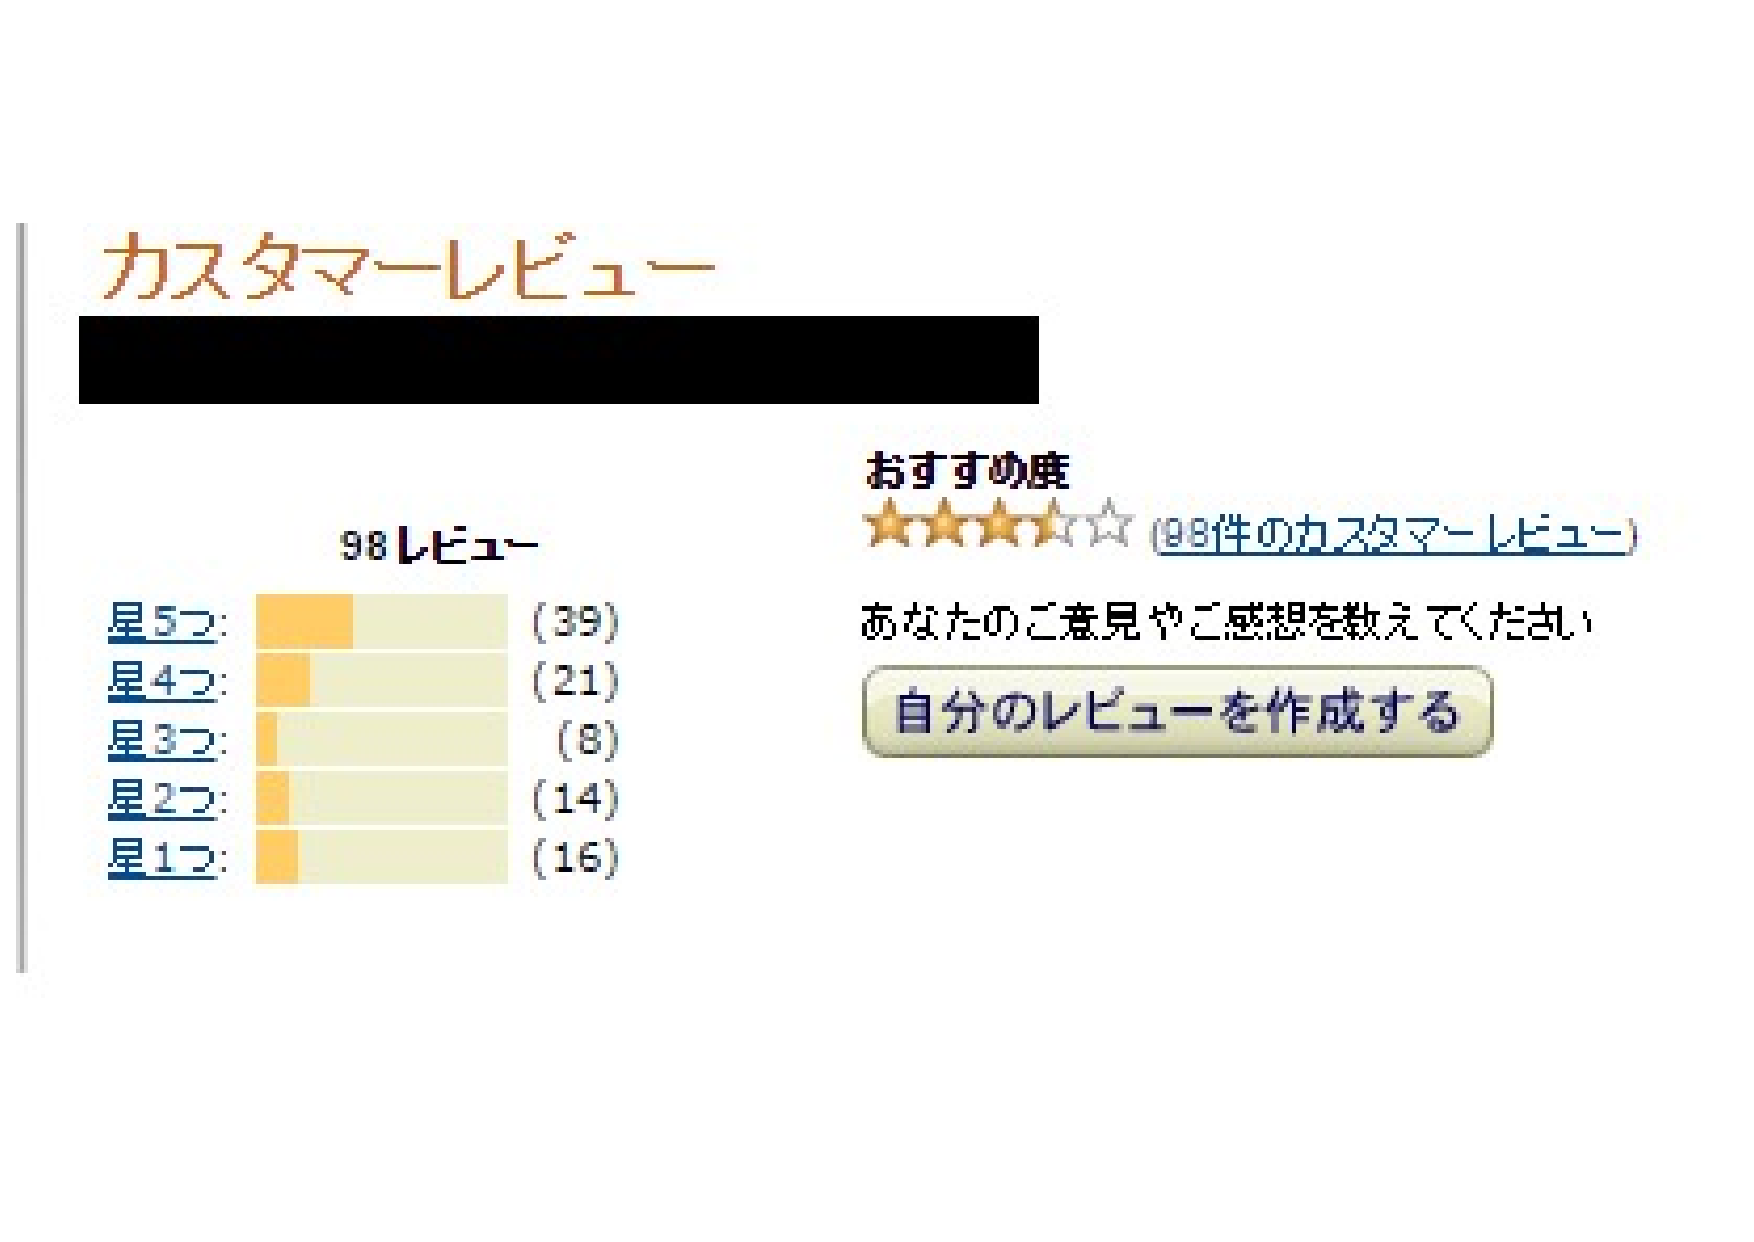
\includegraphics[width=5cm,clip]{customerReview.pdf}
\caption{Amazonのレビューの一例}\label{サンプル図}
\end{wrapfigure}

それらのレビューが実装されている有名なオンラインショッピングサイトでは,利用者が行える内容として商品についてのレビューを記入することや,商品に得点を付けることが可能になっている.一例としてAmazonでは商品の値段,写真などが載せられた紹介ページの後にレビューを5段階評価を星で表現している.最初に大きく5つ星のうちの平均を表示し,その後Amazon独自の方法で最も参考になったカスタマーレビューの順で表示されている.Amazonではレビューを付けた人で統計をして表示しているものはこの平均値しか存在しない.

そこで,レビューを代表付ける表現をしているものが平均しかないことに疑問を感じた.実際には商品とは一切関係のないレビューや明らかに商品に対して理解が足りないレビューがあり,それらのような本来加えるべきでないレビューも多々存在する.そこで平均値よりも参考になる方法を探そうと考えた.
\cite{hattori2011} 
\cite{yamazawa2006}



\section{研究の目的}

新しいレビューの方法をつくりあげることを目的とする.




\section{プロジェクトマネジメントとの関連}

PMBOKにおける10個の知識体系エリアのひとつとして品質マネジメントがある.その内容には
「品質コントロールの最終的な目標は,成果物の正しさを決定することである.」\cite{pmbok2013}
と記述されている.

レビュー評価の信頼性が向上することでオンラインショッピングサイトのレビューを利用したプロジェクトの成果物の正しさを証明しやすくなる.




\section{研究の方法}

\subsection{収集方法の策定}

Amazonにはレビューを見た人に対して参考になったかどうかを判断させるシステムが存在するのでこれを利用することとした.

Amazonのレビューは5段階評価であり.これらの評価値をレビュアーが主観的に判断し,その理由をコメントできる.
その後,レビュアーの評価やコメントを読んだ結果からそのレビューが参考になったかどうかを回覧したユーザに判断させることもできるシステムである.


これらAmazonのレビューデータを集める際に,2つの方法でデータを収集する.


1つめがデータをソフトウェアに手入力で行い計算式を入れていく方法である.
この方法はソフトウェアを使用しているものの,ほぼ手作業なのでミスが生じやすい.
よってある程度データが取れ次第2つめの方法を行うこととする.

2つめがオペレーティングシステムのUbuntuの環境を準備し,必要なデータのみを受信,プログラムに計算を行わせる方法である
この方法を利用することで1つの商品のレビューすべてを一度に受け取ることが可能になり,これにより短時間で多量のデータを取得することが出来る.


\subsection{計算方法の策定}

計算方法は商品1件あたりに存在するすべてのレビュアーの数,レビューごとのの参考になったと答えた比率から割り出すこととした.

具体的には


\[
  重み付き5段階評価 = \frac{5段階評価*\frac{「参考になったと回答した人数」}{参考になる・ならないの判断をした人数}}{\frac{「参考になったと回答した人数」}{参考になる・ならないの判断をした人数}}
\]
このような計算方法を使用した.


\section{現在の進捗状況}


計86件のレビューデータを収集し,そのデータを下に平均五段階評価と重み付き5段階評価の散布図を作成した.

よって発案した計算方法が新しいレビュー方法を作り上げていることに繋がらないので,さらに集計を行い,レビューの特徴を掴み新たな指標を加えていくこととした.

そこで,評価別に「レビュアー数」「参考になる・ならないの判断をした人数」「参考になったと回答した人数」を調査した.

その結果,評価2以下のレビューで参考になったと回答した割合は評価4以上のレビューで参考になったと回答した割合の約1.5倍と判明した.

\section{今後の計画}

現時点では新しいレビュー方法を作り出せていない状況で,集計件数も80件程度と引き続きレビューの集計を行う.

同時にクラスター分析や標準偏差を求めさらに分析を進める.


\bibliographystyle{junsrt}
\bibliography{biblio}%「biblio.bib」というファイルが必要.

\end{document}
